\documentclass{beamer}
\usetheme{Madrid}
\usecolortheme{default}

\usepackage[utf8]{inputenc}
\usepackage{graphicx}
\usepackage{booktabs}


% Title Page Information
\title[Epstein Files Analysis]{Epstein Files Analysis}
\author{Alessandro Gubbiotti}
\institute{Master MIDAS at Elis}

\begin{document}

% --- SLIDE 1: TITLE PAGE ---
\begin{frame}
    \titlepage
    \vfill
    \begin{center}
        
\includegraphics[width=\textwidth,height=3.5cm,keepaspectratio]{Images/DOJ.png}
    \end{center}
\end{frame}

% --- SLIDE 2: BACKGROUND (3 IMAGES, NO WORDS) ---

\begin{frame}{Context}
    \begin{columns}
    
        % LEFT COLUMN — your text/data
        \column{0.5\textwidth}
        % Write your Epstein files data here
        \small
        \begin{itemize}
            \item Key dates:
            \item Legal filings:
            \item Agencies involved:
            \item Public response:
        \end{itemize}
        
        % RIGHT COLUMN — stacked images
        \column{0.5\textwidth}
        \centering
        
        
\includegraphics[width=0.8\textwidth, height=2.5cm]{Images/First_Amandment.jpeg}
        \vspace{0.3cm}
        
        
\includegraphics[width=0.8\textwidth, height=2.5cm]{Images/Foia.png}
        \vspace{0.3cm}
        
        
\includegraphics[width=0.8\textwidth, height=1.9cm]{Images/Quaker_Oats_logo_2017.png}
    	    
    \end{columns}
\end{frame}

% --- SLIDE 3: DATA FORMAT ---
\begin{frame}{The Raw Data Format }
    \begin{center}
        \includegraphics[height=0.7\textheight]{actual_document_screenshot.png}
        \begin{itemize}
            \item Visualizing the source: Redactions, OCR noise, and legal headers.
        \end{itemize}
    \end{center}
\end{frame}
%
%% --- SLIDE 4: DIDACTIC - OCR CHALLENGES ---
%\begin{frame}{Technical Bottleneck: From Pixels to Text}
%    \textbf{The GitHub Problem:}
%    \begin{itemize}
%        \item Most repositories host raw OCR output.
%        \item High error rates in names/dates due to poor scan quality.
%    \end{itemize}
%    \vspace{0.3cm}
%    \textbf{AI Course Reflection (Didactic):}
%    \begin{itemize}
%        \item Convolutional Neural Networks (CNNs) for layout analysis.
%        \item Handling "noisy" text: Why standard Tesseract fails here.
%    \end{itemize}
%\end{frame}
%

% --- SLIDE 5: DATASET & SEMANTIC RELATIONS ---
\begin{frame}{The Dataset}
    \begin{itemize}
        \item \textbf{Method:} Beyond keyword search—parsing semantic relations ($Subject \to Verb \to Object$).
        \item \textbf{Current State of Art:} Many "cooler" LLM-based methods were published during this project.
        \item \textbf{Honest Assessment:} The AI here is "not supercool," but robust for baseline relational extraction.
    \end{itemize}
\end{frame}

% --- SLIDE 6: GRAPH THEORY TRANSITION ---
\begin{frame}{Graphs: Semantic Graph}
    \begin{itemize}
        \item \textbf{Bipartite Start:} People linked to Documents.
        \item \textbf{The Edge Variables:} Weighting connections by frequency and proximity.
        \item \textbf{Dual Graph Transformation:} Treating relationships as nodes to identify hidden structures.
    \end{itemize}
\end{frame}

\begin{frame}{Graphs: The Bipartite Version}
    \begin{itemize}
        \item \textbf{Bipartite Start:} People linked to Documents.
        \item \textbf{The Edge Variables:} Weighting connections by frequency and proximity.
        \item \textbf{Dual Graph Transformation:} Treating relationships as nodes to identify hidden structures.
    \end{itemize}
\end{frame}


\begin{frame}{Graphs: The Dual Graph:}
    \begin{itemize}
        \item \textbf{Bipartite Start:} People linked to Documents.
        \item \textbf{The Edge Variables:} Weighting connections by frequency and proximity.
        \item \textbf{Dual Graph Transformation:} Treating relationships as nodes to identify hidden structures.
    \end{itemize}
\end{frame}
\begin{frame}{Counterterrorism: Finding Paul Revere}
\begin{columns}[T]  % <-- aligns columns at the top 
    % LEFT COLUMN
    \column{0.55\textwidth}
    \vspace{0.2cm}
    Dai dati raccolti in 
    \vspace{0.2cm}
    \includegraphics[width=\textwidth,height=0.9\textheight,keepaspectratio]
    {Images/Paul_Revere_person.png}
    
    \vspace{0.05cm}
    {\tiny Grafo che unisce persone cha appartengono alla stessa associazione }

    % RIGHT COLUMN
    \column{0.45\textwidth}
    
    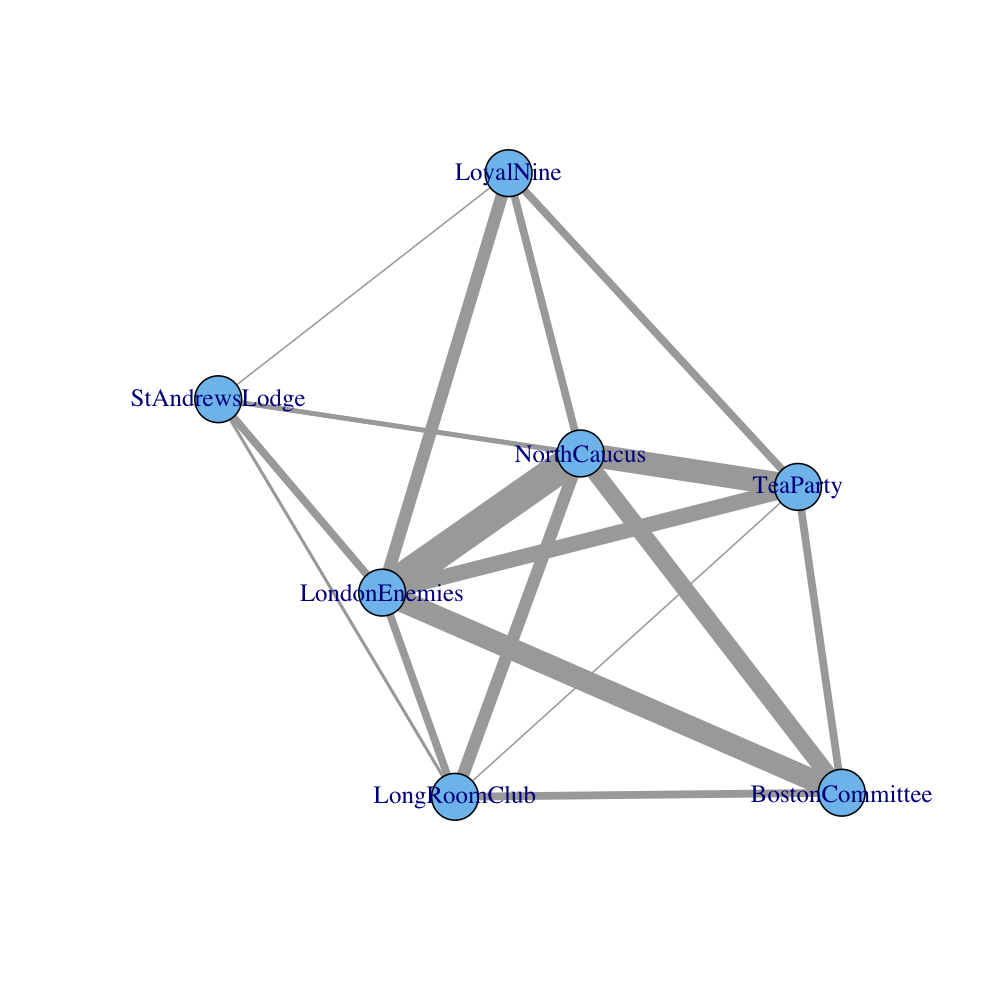
\includegraphics[width=0.75\textwidth]
    {Images/Paul_Revere_Metadata.png}
    
    \vspace{0.05cm}
    {\tiny Dual Graph}
    
    \vspace{0.2cm}
    
    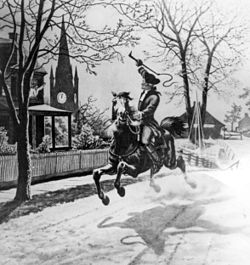
\includegraphics[width=0.60\textwidth]
    {Images/Paul_Revere.jpg}
    
    \vspace{0.05cm}
    {\tiny Paul Revere}

\end{columns}

\footnote{\tiny https://kieranhealy.org/blog/archives/2013/06/09/using-metadata-to-find-paul-revere/}
\end{frame}



% --- SLIDE 8: MASSIVE DISCLOSURES ---
\begin{frame}{Aims 2: The Transparency Context}
    \begin{itemize}
        \item Comparing to the **Panama Papers** or the **Stasi Archives (1989)**.
    \end{itemize}
    \begin{center}
        \includegraphics[height=3cm]{panama_papers.png} \quad
        \includegraphics[height=3cm]{soviet_archives.png}
    \end{center}
\end{frame}

% --- SLIDE 9: CASE STUDIES & IDENTIFICATION ---
\begin{frame}{Distinguere Soggetti: Chomsky vs. Prince Andrew}
        \begin{columns}
        \column{0.5\textwidth}	
	\textbf{Noam Chomsky}
	\vspace{0.3cm}
        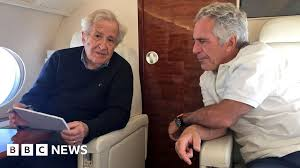
\includegraphics[height=3cm]{Images/Chomsky_Epstein.jpeg} 
        \begin{itemize}
        	\item 
		\item
		\item  
	\end{itemize}
        \column{0.5\textwidth}
       	\textbf{Prince Andrew}
	\vspace{0.37cm}
	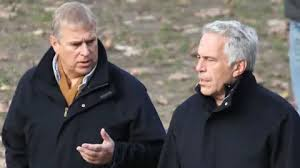
\includegraphics[height=3cm]{Images/Andrew_Epstein.jpeg}  
    \begin{itemize}
	\item 
	\item Esponente di spic
	\item Eroe della guerra nelle Malvine
    \end{itemize}
	\end{columns}
\end{frame}

\begin{frame}[Ma forse]
	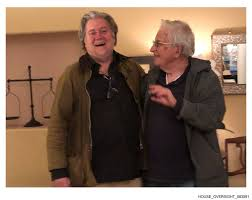
\includegraphics[width=\textwidth]{Images/Bannon_Chomsky.jpeg} 
\end{frame}

\begin{Frame}[Unmasking]
 \textbf{Unmasking:} Triangulating data to identify "Unknown Persons."

\end{Frame}

% --- SLIDE 10: INFORMATION LOSS & LIMITATIONS ---
\begin{frame}{The "Epstein Universe" Constraint}
    \begin{itemize}
        \item \textbf{Conditionality:} Findings are limited to the scope of these specific files.
        \item \textbf{Granularity Mismatch:} Balancing a 100-page deposition against a 2-line email.
        \item \textbf{Lossy Compression:} What is lost when an email becomes a graph edge? (Tone, intent, and subtext).
    \end{itemize}
\end{frame}

\end{document}
